\chapter{Introduction}
Performance of an operating system is crucial as any degradation can significantly
affect the performance of all applications running above it. Moreover, when a
new version is released and it contains a performance regression, it can even
break the stability of business applications leading to great financial losses.
An important part of operating systems is implementation and strategy of a process
scheduler, which manages processes and their processor time.

In the Linux kernel, scheduler used to be simple, but with an introduction of multi-core CPUs came
a requirement for multiple runqueues for each core and their balancing. This brought
some complexity to the code and it took some time to eliminate bugs and tune the
scheduler behavior. Another change came with symmetric multiprocessing technology bringing
to market machines with multiple CPU sockets and non-uniform memory organization
and access. Scheduling on those systems is still under an active development and
therefore it is prone to performance degradation bugs. In order to discover these bugs and to
keep performance of the operating system, performance testing is essential. Due
to this fact, it is essential to evaluate performance of the scheduler before
each release.

Compared to functional testing, performance cannot be evaluated as just true and
false results. It is more challenging as we have to (1) compare it relatively with
previous versions or measurements, and (2) choose a suitable threshold for reporting
the performance regression. Due to complexity of the scheduler, the common tools
for inspecting performance may often yield unsatisfying results.
Moreover, the biggest performance regressions of the scheduler do not dwell in an
inefficient code, but instead in an inefficient placement of processes to the
CPU cores and their queues.

This thesis deals with performance testing of the Red Hat Enterprise Linux
(RHEL) kernel scheduler done in Red Hat, Inc. company.
The usual performance testing method of the scheduler is to simulate load
similar to the real usage. Currently, there are many benchmarks targeting different
types of load, usually spawning many parallel process, sometimes even
communicating between each other. The results of measurements of the performance
must be stored systematically and effectively for later
comparisons. In order to effectively interpret the collected
results and their comparisons, their visualization of various kinds is essential.

In this thesis, we propose new way of interpreting long-term results of the
benchmarks using box plot graphs in order to enhance the process of data
analysis. This visualization should help with inspecting the measurement
stability of benchmarks and with finding versions where performance degradations
appeared or were fixed.

Moreover, to help to reduce time one has to spend analyzing comparisons,
we propose an utilization of machine learning methods that will
automatically check for possible degradations in the Linux kernel scheduler. We will
describe creation of a dataset for classification, compare different
classifiers, and evaluate their accuracy on the dataset.

This thesis is structured as follows. In Chapter \ref{ch:scheduler} we describe
Completely Fair Scheduler -- the current process scheduler of the Linux kernel,
architecture of symmetric multiprocessing systems, and how the scheduler handles
them. In Chapter \ref{ch:measurement}, we describe the performance measurement of
the Linux process scheduler. First we introduce benchmarks used in Red Hat for
load testing of the scheduler performance and then we describe complementary tools for analysis of
behavior of the scheduler and of the system. Ways of storage of the collected data
and their visualization for comparison are described in Chapter
\ref{ch:processing}.

We propose a new way of visualization of long-term results comparison called
\emph{Timelines} in Chapter \ref{ch:timelines}. In Chapter
\ref{ch:ai}, we propose utilization of machine learning methods for automatic
classification of comparison of two results to recognize a performance
regression.



\chapter{Linux process scheduling} \label{ch:scheduler}
Scheduler is a part of an operating system which assigns the processor time to tasks.
Its main goal is to maximize effectivity of the CPU usage and to ensure fairness of the
CPU time assigned to each task.

There are two opposing targets for a scheduler: either maximizing the throughput or
minimizing the latency. Lower amount of context switches leaves more CPU time for
tasks, but raises the response time on system events.
While users' workstations aims for a low response time, computational servers
require high throughput. Scheduler can then be usually tuned to fit the intended
purpose.

In this chapter we describe basic behavior of Linux process scheduler. Then we
compare uniform and non-uniform memory access on multiprocessor architectures
and how scheduler handles them.

\section{Completely Fair Scheduler}
Completely Fair Scheduler (CFS) is the current Linux process scheduler, which was
merged into the version 2.6.23 of the Linux kernel in 2007. Its author is Ingo
Molnár, who is the author of the previous \emph{O(1) scheduler} as well.

CFS features queuing tasks in a red-black tree structure ordered by time spent
running on the CPU so far. Red-black tree is a binary search
tree with self-balancing mechanism based on marking nodes with either red or
black color. When the scheduler needs to choose the next task to run, it takes
the leftmost node with the lowest execution time.

The time complexity of the CFS scheduling is O(log N), where N is the number
of running tasks. Taking the leftmost node
with the next scheduled task can be done in a constant time, but queuing the task
requires O(log N) operations to insert it back into the red-black tree. Even
with a higher scheduling complexity, the CFS scheduler has a better fairness and
responsiveness than the previous O(1) scheduler, which used a simple queue to
choose the next task.
% CFS can also handle priority better: it requires only one queue instead of two
% for each of 140 priorities in Linux for O(1)

On multi-core systems, the scheduler uses a separate queue for each core. In
order to effectively use the processing power, the scheduler must regularly
balance those queues by moving processes from the most busy cores to idle ones.

When moving processes between cores, scheduler takes in the account a topology
of the system. Losing data from caches after the migration can have a bigger
impact on performance than leaving the process on the busy core.

% Linux kernel book
CFS solves this problem by using scheduling domains. Scheduling domain is a set
of CPUs that should be balanced between themselves. CPUs in a scheduling domain
are divided into groups. Scheduler then checks the load of the whole groups to
decide if there is a need to migrate processes between them.

There are multiple levels of scheduling domains with different parameters such as
how often is the load difference checked or how big the load difference between
groups must be to migrate tasks to balance the queues.
The lowest level is between hyper-threaded logical cores where there are almost
no losses of cached data and rebalancing can be done quite often.
A higher level is between physical processor cores where cache losses can have
bigger impact on the decision to migrate the task.
Above those cores can be processor sockets on machines with multiple physical
processors with different access speed to different memory sections.

Scheduling domains are regularly rebalanced by going up from bottom of the
scheduling domain hierarchy and by checking balance of the groups on each level.

% https://lwn.net/Articles/764482/
\begin{figure}
  \centering
  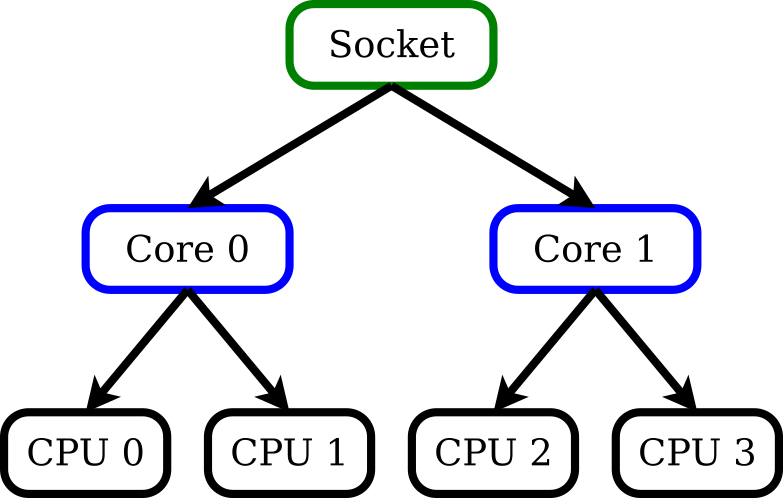
\includegraphics[width=4cm]{sched-domains}
  \caption{Hiearchy of scheduling domains\cite{sched-groups-lwn}}
  \label{fig:sched-dom}
\end{figure}

\section{Scheduling on SMP systems}
Symmetric multiprocessing (SMP) is an architecture of computers with multiple
physical processors that have a single shared memory, a shared access to all IO
devices, and that run on the same instance of operating system. This allows the
machine to offer more processing power with a little overhead caused by memory
sharing.

Each processor has still its own high speed cache, but due to memory sharing,
\emph{cache coherence} must be maintained -- the data shared between processors
in their caches must be uniform.

There are two ways of accessing the shared memory from multiple processors:
uniform (UMA) and non-uniform (NUMA) memory access. When correctly used, the
NUMA technology has higher performance capability with similar configuration
compared to UMA systems. In our experience most paying customers of Red Hat use
the NUMA technology and we will primarily focus on scheduler behavior on this
SMP architecture.

\subsection{Uniform memory access}
In the UMA architecture, all processors share a single memory controller that
they use to access the shared memory. Therefore, each processor has the same
speed of memory access and the same latency. They share a common access route to
the memory, which brings more simplicity at the cost of a lower bandwidth and
speed.

In this architecture it is easier for the scheduler to balance processes
between the physical processors. The time to access the shared memory is the
same on all of the cores and therefore there is no need to move the memory
associated with a process to any other place for faster access.

\subsection{Non-uniform memory access}
The NUMA architecture tries to solve the problem with low bandwidth.
It arranges physical processors or cores into nodes, where each node has its
own separate memory and a bus for faster access. This significantly improves
overall memory throughput of the system when used correctly.

Nodes also have to be connected to each other to access memory of other
nodes. That is achieved using either interconnecting buses or controllers. Each
manufacturer has its own technology implementing the interconnection: Intel uses
Ultra Path Interconnect which replaced its QuickPath Interconnect from older
machines. On the contrary AMD uses Infinity Fabric supersetting the older
HyperTransport.

On bigger machines with a large amount of processors, not every two processors
are necessarily connected. Instead, they may access the data through a path
of connected nodes. This can be seen in Figure \ref{fig:proliant} showing an 8
NUMA node machine with an advanced structure of interconnect buses and
controllers.

%Best Practices When Deploying Linux on DL980 4AA3-6556ENW.pdf
\begin{figure}
  \centering
  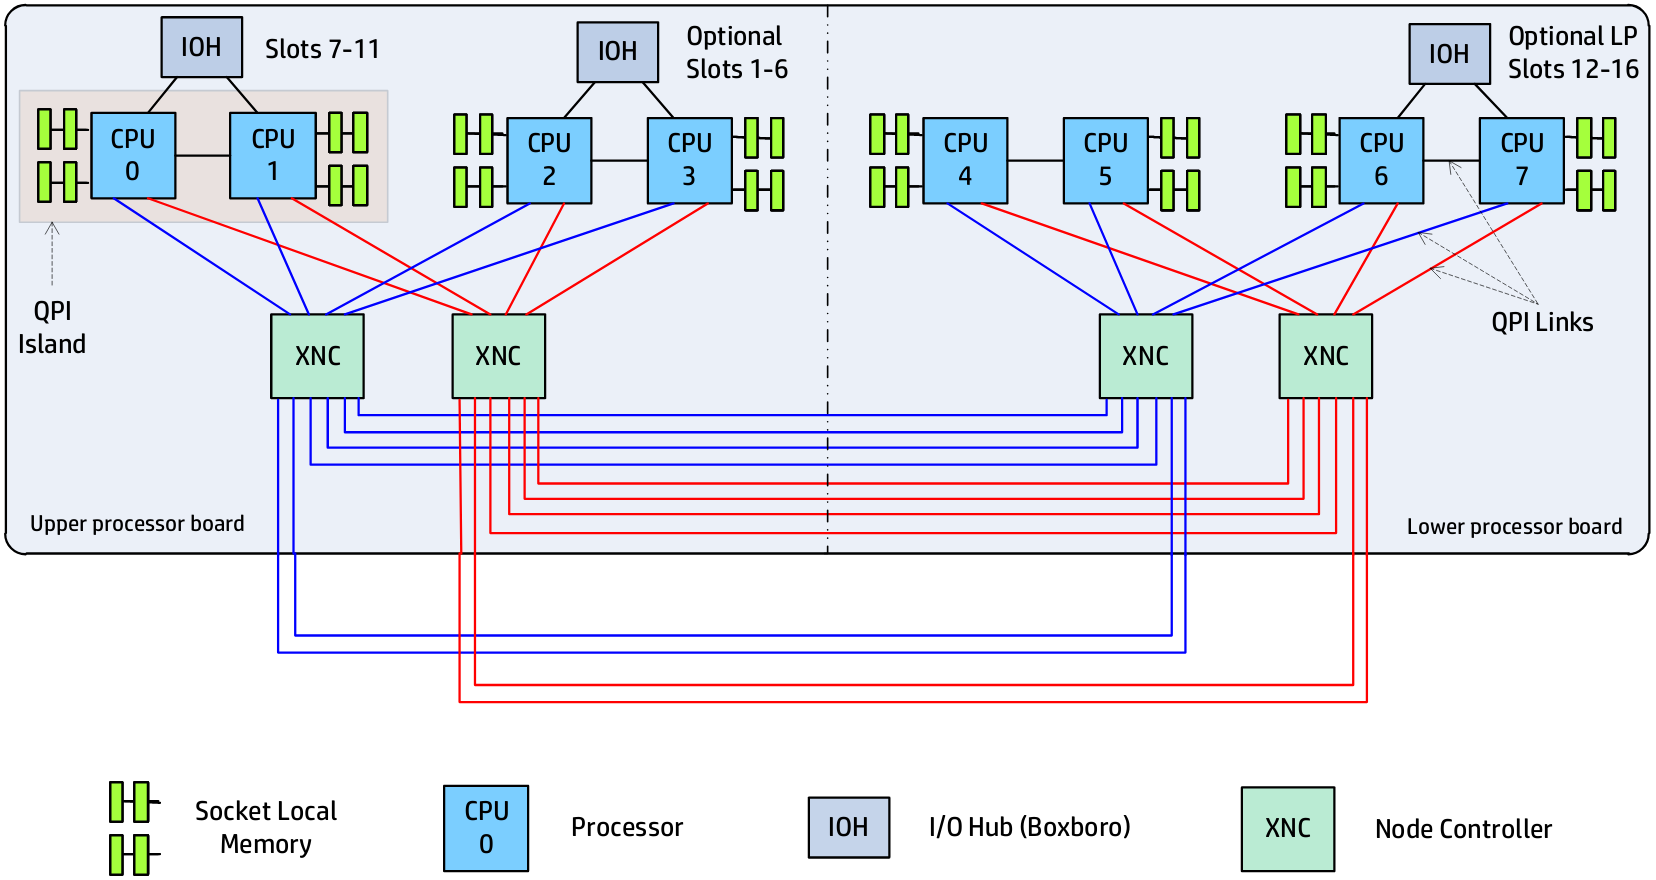
\includegraphics[width=14cm]{proliant}
  \caption{Architecture of NUMA communication on HP ProLiant
    DL980\;\cite{proliant}. Each processor connected with its own local memory
    makes up a NUMA node. Each pair of nodes have dedicated interconnect bus for
    faster data transfer between them. Communication with other nodes is
    realized through node controllers. The topology of the interconnect buses
    shows there will be 4 different access speeds depending on the distance
    between nodes. The local access is the fastest, then follows the access to
    the neighbor node, the access through one controller and the slowest is the
    access through both controllers. The interconnect buses are doubled to avoid
    overloading one of them.}
  \label{fig:proliant}
\end{figure}

Consequence of interconnection between NUMA nodes is the different latency
between nodes which must be taken into account when balancing tasks between
nodes. Difference in the access latency between a pair of NUMA nodes for the
machine from Figure \ref{fig:proliant} can be seen in the following part of
output from a command \verb|numactl --hardware|:

\begin{minipage}{\linewidth}
\begin{verbatim}

node distances:
node 0 1 2 3 4 5 6 7
0: 10 12 17 17 19 19 19 19
1: 12 10 17 17 19 19 19 19
2: 17 17 10 12 19 19 19 19
3: 17 17 12 10 19 19 19 19
4: 19 19 19 19 10 12 17 17
5: 19 19 19 19 12 10 17 17
6: 19 19 19 19 17 17 10 12
7: 19 19 19 19 17 17 12 10
\end{verbatim}
\end{minipage}\\

Balancing tasks between NUMA nodes is difficult for the scheduler since it needs
to take into account an expensive memory movement or access to different nodes.
With a wrong approach the performance of a NUMA system can drop even below the
performance of a similar UMA
system\footnote{http://highscalability.com/blog/2013/5/30/google-finds-numa-up-to-20-slower-for-gmail-and-websearch.html}.

Balancing processes between NUMA nodes is still in active development, which
brings many changes. These usually improve performance, however, there are cases
when a change can cause a performance regression. Therefore, it is essential to
carry out a thorough performance testing of the scheduling.

% TODO task can be pinned



\chapter{Performance measurement} \label{ch:measurement}
Performance testing is examination of the system behavior under a workload and of its
effectivity of resource usage. For many systems, the time they are able to
respond in is crucial and this property affects the usability of the system.

Compared to functional testing, performance testing does not produce an exact true
or false result. It produces a set of numerical values which must be compared to
pressumed values or values from an other version to make a conclusion.

After the performance measurement, the next step is inspection of behavior of
the system to understand the measured values and to determine the causes of the
difference from the expected values.

In order to measure the performance of scheduler, we use benchmarks.
Benchmarks generate artificial load imitating the load in real environment.
While stress testing the system they also measure its performance. The benchmarks
typically return a value representing the performance of the system. The value
is usually in the form of the time that the task needed to finish or of the amount of
the operations that the system could perform per a unit of time.

In previous chapter, we have introduced the current state of task scheduling in
Linux kernel.
Effectivity of the scheduling and of their migration between processors affects
the amount of the tasks that the system can handle and the time that a task
spends before finishing.

Although the available benchmarks generate values that are suitable for comparison, they
do not provide any more detailed information about how the system achieved the
measured performance or where the possible bottlenecks could be.

To get a better insight into the behavior of the system, there are many tools to
collect performance records about the system behavior. Useful information about the
scheduler include assignment of tasks to the processor cores, the time that the
tasks spent out of the CPU in queues, load of each processor core or the
location of memory of the processes on NUMA systems.
% TODO cite http://www.brendangregg.com/activebenchmarking.html

\section{Performance metrics} \label{sec:metrics}
\paragraph{Throughput} metrics represents the amount of operations per time
unit. It can use different units: floating point operations, operation as
a specific tasks defined by benchmark (e.g. SPEC Java benchmarks) usually
executed per second. Higher values mean better performance.

\paragraph{Run time} is simply the real time the benchmark needed to finish the
execution. It is mostly presented in seconds, but longer runs can be presented
more human-friendly converting the time to hours, minutes, and seconds. The
lower the run time is, the better performance it represents.

\paragraph{Time out of CPU} represents the time the benchmark spent in process
queue waiting for execution. This metric can be calculated from user, kernel and
real time provided by \emph{time} utility and number of threads, that the
application used:
$$T_{out\_of\_cpu} = (T_{real} \times used\_threads) - (T_{user} + T_{kernel})$$
The lower this value is, the better behavior of scheduler it represents.

\section{Benchmarks}
In the following section we will describe the benchmarks that are currently used
to evaluate performance of the latest kernel versions. The benchmarks are
usually based on real applications used both in scientific and in business
environments and are meant to stress test the system.

The benchmarks run in many threads or processes and feature communication
between them to utilize communication between processors. A bad distribution of
processes and threads by the scheduler increases their time of waiting in the
queue to rise and the performance of the system naturally goes down. Moreover,
on NUMA systems, the performance depends also on placement of data in the
memory.

\subsection{NAS Parallel Benchmarks}
NAS Parallel Benchmarks\;\cite{nas-parallel} is a set of programs focused on
performance of highly parallel computations on supercomputers. In addition to
floating point computations, it targets communication and data movement among
computation nodes. The performed algorithms are based on large scale
computational fluid dynamics at the Numerical Aerodynamic Simulation (NAS)
Program which is based at NASA Ames Research Center.

Benchmarks are written in Fortran-90 or in C language, as these were the most
commonly used programming languages in scientific parallel computing community
at the time when the benchmarks were created. They can be compiled with
different classes of problem sizes to suit machines with different amount of
memory and of computational power.

The main output value of the benchmark is the throughput measured in units
called Mop/s (millions of operations per second) representing the amount of
floating-point operations per unit of time.

The benchmark also offers a few parameters that can be passed to the benchmark
before the execution. One of them is the number of computation threads, which in
a lower amount slows down the run time, but allows one to measure behavior of
the system without full usage. Figure \ref{fig:nas} shows an example of a
throughput with different number of threads on a machine with 24 physical cores
and hyper-threading.

The downside of this benchmark is it can only run with a fixed dataset, but not
for a fixed time period. This constraint makes the run time of the benchmark
with less threads longer.

\begin{figure}
  \centering
  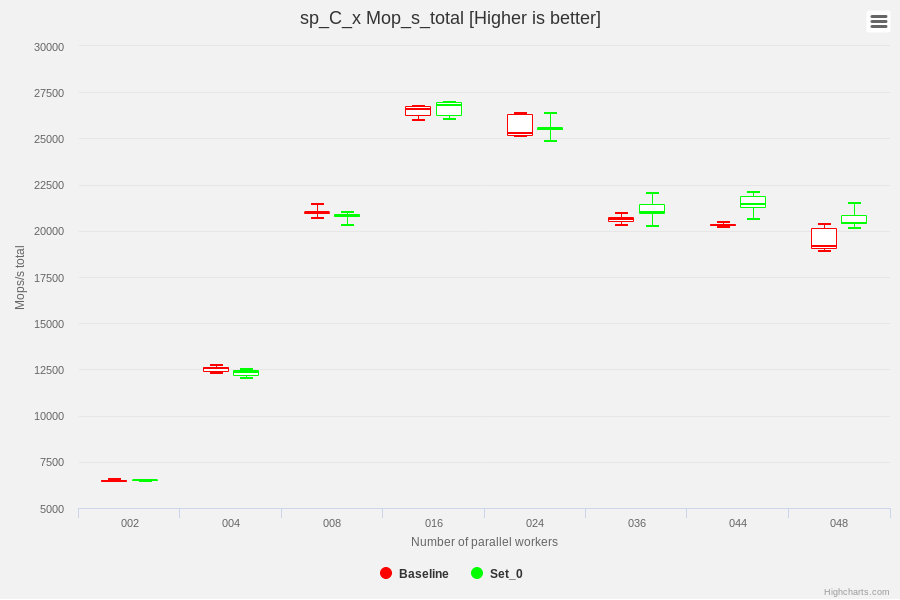
\includegraphics[width=12cm]{nas}
  \caption{Example of Scalar Penta-diagonal solver results from NAS Parallel
    benchmark with different number of computational threads. The size of the
    boxes represent the inaccuracy of measurement caused by noise and
    non-deterministic behavior of scheduler.}
  \label{fig:nas}
\end{figure}

\subsection{SPECjbb2005}
Java Business Benchmark behaves as a server-side Java application. It is
primarily focused on measuring performance of Java core implementation, but it
also reflects a performance of operating system and of the CPU itself. It models
a system of a wholesale company as a multitier application. The benchmark itself
creates the load, measures the throughput, and also generates a simple report in
HTML and raw text formats.

The main output value is \emph{throughput} measured in units called
\emph{SPECjbb2005 bops} \footnote{Business operations per second}. In case we
use more JVM\footnote{Java virtual machine} instances, there is a second unit
called SPECjbb2005 bops/JVM representing an average throughput of a single JVM
instance. The collected metric is memory consumption, which is not that
important for scheduler performance monitoring.

\subsection{SPECjvm2008}
SPECjvm2008 is benchmark primarily focused on performance of Java Virtual
Machine, but its results can reflect performance of the scheduler.

\subsection{LINPACK benchmark}
LINPACK Benchmark\cite{linpack} comes from LINPACK package, which was used to solve systems of linear equations in single or double precision.

\subsection{STREAM benchmark}
The STREAM benchmark is a simple, synthetic benchmark designed to measure the sustainable memory bandwidth (in MB/s) and a corresponding computation rate for four simple vector kernels.
STREAM runs on each core of a mode using the OpenMP programming paradigm. Four synthetic computational kernels are run, and the best rates observed are reported for each choice of thread count.

\section{Performance analysis tools}

\subsection{time}
Time is a simple command for measuring the time that an application spends
running. The most common numbers it reports are the total real time that the
application needed to finish, the time that it spent in the user mode, and the
time spent in the kernel mode.

Many benchmarks provide the execution time themselves which can make this
utility unnecessary. However, the interesting metric is the time that the
application spent out of the CPU waiting in queue. This value is not provided
directly, but provides user, kernel and real time from whose the metric can be
calculated as described in Section \ref{sec:metrics}.

It can be confused with the Bash builtin command \texttt{time}, which provides similar
output, but the real binary can provide more verbose information with
the possibility of custom formatting of output. It can be usually called from
\texttt{/usr/bin/time}.

\subsection{ps}
Ps is a Linux command, which is used to display information about active processes. Its name
stands for ``processes status''. It can provide various information obtainable from
the virtual files in \texttt{/proc} directory. The most common information
include the process PID, time spent on processor, state of the process, used memory,
associated terminal, the command that started the process and more.

Especially useful are the optional columns \texttt{PSR} and \texttt{NUMA}. They
show the number of the processor and the number of the NUMA node where the process is
running. Continuous monitoring of those values can provide view on migration of
the process during its run time. 

Output of the command can be filtered in many ways. By default, it shows only
processes for the current user and for the current terminal, but it can list all
the processes on the system. The listing can be filtered using parameters by
most of the columns of information it provides. The listing can be limited for
instance by a specific terminal, by an effective user, by children of a specified process,
or by a PID a to single intended process.

\subsection{mpstat}
This Linux command provides continuous information about utilization of CPUs. It
can show utilization of processor cores, of NUMA nodes, or of the whole system
dependent on passed argument. Some of the provided values are utilization in
user space, utilization in kernel space, percentage of waiting for IO
operations, percentage of handling interrupt requests and the idle percentage,
when system is idle and does not wait for any IO operation.

Mpstat can collect those data once when executed or at regular time intervals.
The regular collecting of utilization of the CPU cores or of the NUMA nodes is
done through the run time of benchmark. With little processing of the data, it
is easy to watch the distribution of load between the cores and the NUMA nodes
is equal or not.

\subsection{turbostat}
This tool provides measuring of hardware properties of the CPUs with x86
architecture. It reports for each core its usage, frequency, temperature and
percentage of time in idle states. For each socket it reports its power consumption.

There are two ways to run turbostat. It can be supplied with a command to run
and it will return the average values from the run time of the command. Without
the command it will collect the statistics at regular time intervals.

Data from this tool can be used to analyze performance drop caused by the CPU
itself. This can happen due to frequency drop because of overheating or of
missing workload. The power consumption data can be used to roughly compare the
power efficiency of both the scheduler and the physical CPUs, but the command
only provides consumption of the CPUs and their RAM and not of the whole
machine.

\subsection{perf}
Linux tool for monitoring hardware and software events, profiling and tracing.

\subsection{numa* tools}
numactl
numatop
numastat



\chapter{Processing of results} \label{ch:processing}
Results must be stored and visualized.

\section{Storage of the results}
Benchmarks sometimes generate long human-readable output in text or even HTML
format. This is useful when analyzing single report. In the output there are details
of the test run itself, simple resource usage or success of result validation.
However, the amount of result starts to rise with repeated runs, different
amount of instances and new versions kernels.

For the comparison of performance results, the number representing throughput or
time of each benchmark run is usually enough. Those numbers can be preprocessed
from the benchmark output files to a format more suitable for quick accessing
required data.

\subsection{XML files}
XML is a markup language, that can store heterogeneous data in tree structure.
The tree structure can effectively represent the test scenario running each
benchmark operation with different parameters and multiple repetitions.

Another feature of XML format is human-readability offering quick insight to stored
data just with any text editor.
This comes with a disadvantage of redundant data in form of repeated names of
tags and attributes which often take more space than the data itself. Parsing of
the data also take considerable amount of CPU time prolonging the duration of
analysis.

% TODO in our team we use this method for cases described in following figures

Example of results from one run of the NAS Parallel benchmark scenario stored in
XML format is in Figure \ref{fig:xml_result}. Example with aggregated
data is in Figure \ref{fig:xml_sums}. In XML format are stored also properties
of the benchmark run result shown in Figure \ref{fig:xml_config}.

\begin{figure}
  \small
  \begin{verbatim}
<?xml version="1.0"?>
<beaker_run_result>
  <test_result>
    <nas_result benchmark_name="mg_C_x">
      <threads number="2">
        <result mops="5560.4" real_time="31.0" out_of_cpu_time="0.9"/>
        <result mops="5411.4" real_time="32.2" out_of_cpu_time="1.6"/>
        <result mops="5499.3" real_time="31.4" out_of_cpu_time="0.6"/>
        <result mops="5407.4" real_time="31.9" out_of_cpu_time="1.3"/>
        <result mops="5376.1" real_time="32.0" out_of_cpu_time="0.7"/>
      </threads>
      <threads number="4">
        <result mops="10254.9" real_time="16.8" out_of_cpu_time="1.2"/>
        <result mops="10075.4" real_time="17.1" out_of_cpu_time="1.7"/>
        <result mops="10226.6" real_time="16.8" out_of_cpu_time="1.4"/>
        <result mops="10250.2" real_time="16.8" out_of_cpu_time="1.3"/>
        <result mops="10227.7" real_time="17.0" out_of_cpu_time="2.5"/>
      </threads>
...
\end{verbatim}
  \normalsize
  \caption{This example shows beginning of XML file with important values from one NAS
    Parallel benchmark run scenario. The XML file starts with root element
    \texttt{<beaker\_run\_result>} and \texttt{<test\_run>} node which are wrapping
    \texttt{<nas\_result>} nodes representing results from each benchmark operation
    from NAS Parallel benchmark suite. Each benchmark operation is run with
    different amount of threads in few loops to lower the measurement inaccuracy.
    Nodes of results with the same number of threads are wrapped in
    \texttt{<threads>} node. All the values are stored as attributes of the
    corresponding node.}
  \label{fig:xml_result}
\end{figure}

\begin{figure}
  \small
  \begin{verbatim}
<?xml version="1.0"?>
<beaker_run_result>
  <test_result>
    <nas_result benchmark_name="mg_C_x">
      <threads number="2">
        <mops mean="5450.9" stdev="68.4" first_q="5407.4" median="5411.4"
          third_q="5499.3" max="5560.4" min="5376.1"/>
        <total_time mean="31.7" stdev="0.4" first_q="31.4" median="31.9"
          third_q="32.0" max="32.2" min="31.0"/>
        <out_of_cpu_time mean="1.0" stdev="0.4" first_q="0.7" median="0.9"
          third_q="1.3" max="1.6" min="0.6"/>
      </threads>
      <threads number="4">
        <mops mean="10207.0" stdev="66.8" first_q="10226.6" median="10227.7"
          third_q="10250.2" max="10254.9" min="10075.4"/>
        <total_time mean="16.9" stdev="0.1" first_q="16.8" median="16.8"
          third_q="17.0" max="17.1" min="16.8"/>
        <out_of_cpu_time mean="1.6" stdev="0.5" first_q="1.3" median="1.4"
          third_q="1.7" max="2.5" min="1.2"/>
      </threads>
...
\end{verbatim}
  \normalsize
  \caption{Another form of stored data shows this beginning of XML file. Instead
    of all values obtained from the benchmark run scenario, here are only
    aggregated statistical values form the sets of collected values from each
    configuration. The aggregated values include minimum, maximum, mean, median,
    quartiles and standard deviation of metrics like throughput, run time, or
    time in queue for CPU. Those values are directly usable for plotting of
    comparison graph without any manipulation with them lowering the time for
    generation of reports.}
  \label{fig:xml_sums}
\end{figure}

\begin{figure}
  \small
  \begin{verbatim}<?xml version="1.0"?>
<beaker_run_result>
  <settings>
    <BenchmarkName value="NASParallel"/>
    <Distribution value="RHEL-7.5"/>
    <Kernel value="kernel-3.10.0-862.el7.x86_64"/>
    <Architecture value="x86_64"/>
    <TunedProfile value="throughput-performance"/>
    <SELinux value="Enforcing"/>
...
\end{verbatim}
  \normalsize
  \caption{Example of XML file storing properties of benchmark run results.}
  \label{fig:xml_config}
\end{figure}

\subsection{Relational database}
Relational database is a type of database using relational model. The relational
model stores data in tables using rows for records and columns for their
attributes. Each row represents an unique record with its attributes in columns.
Columns store values of attributes with same data type. Record in different
tables can be connected in relationships.

There are many database management systems implementing the relational database
model available under various licenses. From the open-source we can name
PostgreSQL, SQLite, MySQL, or its fork MariaDB. To the category with proprietary
code belong implementations from companies including Oracle, Microsoft, or IBM.

Data in database are managed using SQL (Structured Query Language). It provides
commands for storing, manipulating and retrieving data. With advanced joining of
tables and filtering it provides wide possibilities of data processing just at
the point of reading of the stored data.

Database offers much faster access to data without complicated parsing of text
files. Searching through the data can be much faster with indexing of the
records by selected columns. Moreover, databases store data more
space-efficiently directly in binary format to avoid unnecessary conversions.

The efficiency of database comes with its disadvantages. 
Storing the data in binary form eliminates the possibility of quick insight to
data like with XML files. To access any data is required to write SQL query to
request specific from the storage.
More complications come with design of the database tables. Different benchmarks
produce different type of result and the requirements for stored data can change
over time. This requires building universal complex structures or occasional
changes in the database model.

In our team we consider the option of storing results of the benchmark in
database, considering the work needed for migration from storing in XML files.

\section{Visualization the results} \label{ch:visualization}
Effective analysis of results from performance measurement requires delivering
the comparison in a form in which can human quickly see the differences of
measured values and their severity. Visualization offers this advantage against
raw text data collected from benchmarks and performance analysis tools.

velké množství dat  na malém prostoru  ve srozumitelné formě
effectivity against text representation
reveals relations between values
utilization of human image memory

It must deliver easily understandable data even to people that do not work with
performance analysis on their daily basis.

\subsection{Line graphs}
Line graphs are the simplest method of displaying a course of values of variable
dependent on a parameter in two dimensional space. It allows to easily spot
nature of the plotted values -- either rising, descending or constant. The
data can be plotted as discrete values using points or as a continuous function
using a line. Comparison of more variables from different datasets is done by
plotting multiple lines to the same graph, one for each variable. In Figure
\ref{fig:linegraph} is example of line graphs showing CPU utilization of system
NUMA nodes and ratio of access to memory of remote nodes.

Although line graphs are quick and simple to create and use, they fail to scale
for larger amount of lines in single graph. Larger amount lines become too
confusing and impossible to read. Graphs of CPU usage of each NUMA node in
Figure \ref{fig:linegraph} is still readable, but impossible to use for
utilization of every CPU core.

\begin{figure}
  \centering
  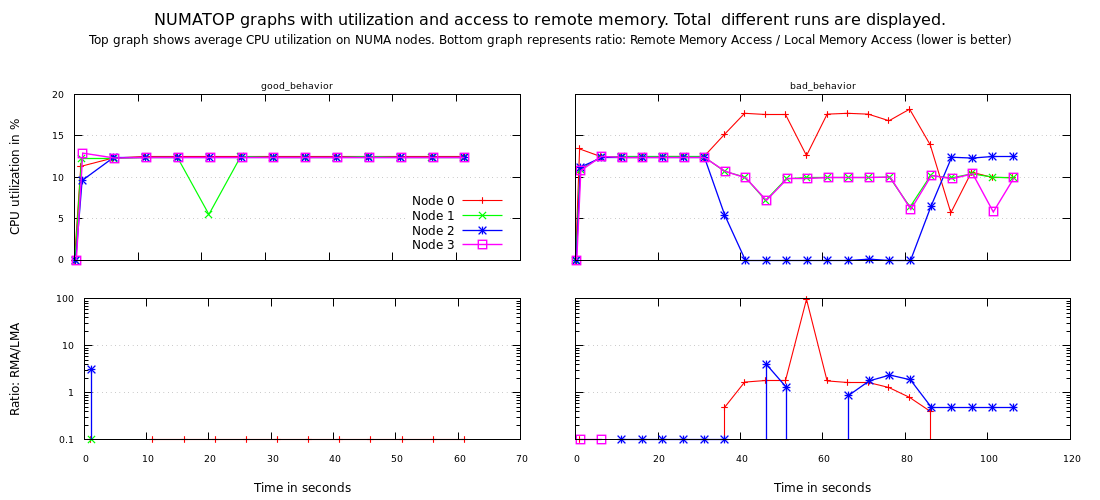
\includegraphics[width=14cm]{numa_behavior}
  \caption{Example of line graphs showing statistics collected using numatop
    utility. The graphs in top row show CPU utilization of each NUMA node
    through time and in the bottom row show ratio of access to local memory of
    the node and memory of remote nodes. The graphs on the left show expected
    behavior of scheduler causing uniform utilization of each node and minimal
    amount of access to memory of remote nodes. The utilization graphs use
    linear y axis and memory access graphs use logarithmic y axis. The plotted
    values were collected on 4 NUMA node machine under workload from NAS
    Parallel benchmark running in 4 threads.}
  \label{fig:linegraph}
\end{figure}

\subsection{Heat maps}
Heat maps are three dimensional graphs which are using color as the third
dimension for values. This allows to plot two dependencies of the values
compared to line graphs, which must use multiple lines to plot the same data.
Heat maps provide better scalability for larger data, where line graphs would be
confusing with too many lines. It is also much easier to spot correlation
with the additional dimensions compared to line graphs.

In the Figure \ref{fig:heatmap} is heat map showing utilization of all CPU cores over
time under workload. The data were collected by mpstat utility and processed to
show sum of user and kernel space utilization of each core. Plotting those data
using line graph with a line for every core would be confusing even for this
relatively small amount of CPUs.

\begin{figure}
  \centering
  \includegraphics[width=14cm]{heatmap}
  \caption{Example of heat map showing CPU utilization over time. The machine
    with 24 logical CPUs is under workload from NAS Parallel benchmark running
    in 16 threads.}
  \label{fig:heatmap}
\end{figure}

Another use of heat map is shown in Figure \ref{fig:numa_heatmap}. It does not
show utilization of threads, but their location on which NUMA node collected by
ps utility. This heat map shows the migration of threads between NUMA nodes and
the expected result is not the highest value, but minimum of color changes in
each line. The shown data comes from NAS Parallel benchmark, which was run with
16 and 24 threads in 5 loops. The heat map shows better scheduler behavior on
the 16 threads run than on the 24 threads run.

\begin{figure}
  \centering
  \includegraphics[width=14cm]{numa_heatmap}
  \caption{Example of heat map showing thread migration between NUMA nodes. The
    expected result is not the highest value, but minimum of color changes in
    each line. The shown result comes from machine with 24 logical CPUs running
    NAS Parallel benchmark on 16 and 24 threads in 5 loops.}
  \label{fig:numa_heatmap}
\end{figure}

\subsection{Box plots}
Box plot is a method for displaying statistical properties of data from multiple
measurements. It extends the simple visualization of discrete values by adding
to the median values also the minimum and maximum measured values and first and
third quartiles from the measurement. In special cases are also added marks for
99\textsuperscript{th} or similar percentile relevant for the given case.
% TODO why it displays those values

All the displayed values shows the accuracy and reliability of measurement. This
insight helps to distinguish real performance regression from noise caused by
unpredictable behavior of the scheduler and measurement error.

In the Figure \ref{fig:boxplot} is an example of box plot showing throughput
measured by NAS benchmark with different number of threads.  

\begin{figure}
  \centering
  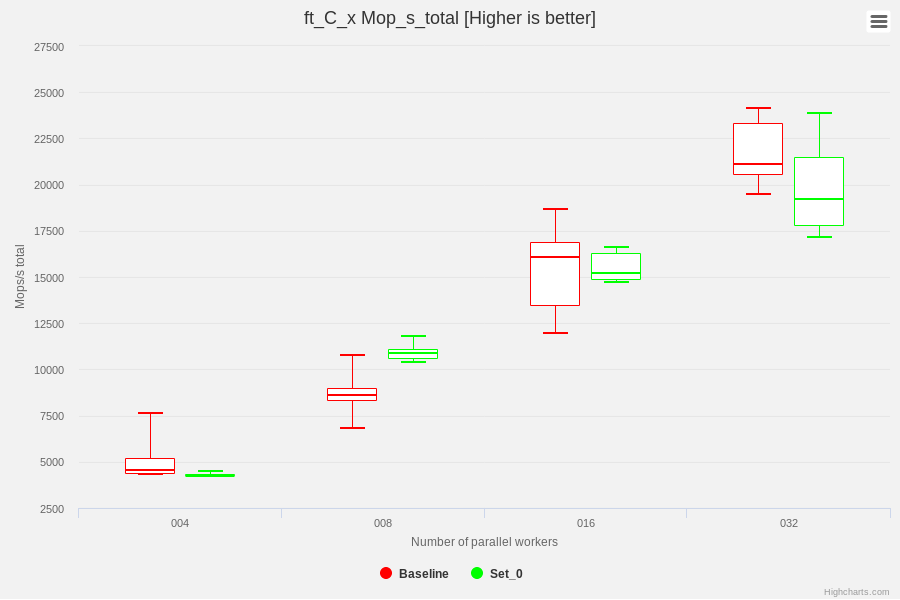
\includegraphics[width=12cm]{boxplot}
  \caption{Example of boxplot showing throughput measured by NAS benchmark from
    multiple measurements with different number of threads.}
  \label{fig:boxplot}
\end{figure}



\chapter{Visualization using timelines} \label{ch:timelines}
A common way to analyze performance reports is to compare two results measured
for different versions or settings. Usually, these
are called baseline and target results or profiles. The comparison of two
results allows one to
interpret many details about the measurement and changes between versions. Those
details usually contain clues to the cause of possible performance changes.

However, sometimes it is not enough to compare just two strictly following
versions. If instead we analyze larger amount
of results over longer period of time we can see a new perspective. In that case
there is much
more visible difference between the deviation from measurement error and the
performance change. It is also easier to find the versions, where exactly a
performance degradation occurred and where was fixed.

With larger amount of data, we can also detect creeping performance drops, which
appeared continuously over longer period of time and could not be detected,
because they were within the tolerance due to the measurement deviation.

This chapter proposes creation of reports with comparison of multiple results of
performance measurement from benchmarks used in out team in Red Hat. The
visualization of course of performance results will help to see the performance
of Linux kernel scheduler in wider range of time and help to determine stability
and precision of different benchmarks.

\section{Design}
Main purpose is to watch performance through kernel versions on a specific testing
machine. Output of the timelines generator will be HTML reports showing
benchmark results of desired kernel versions on single machine. Mockup of
produced HTML page is described in Figure \ref{fig:mockup}. Displayed results
will be specified using rules for base kernel as the first reference result
and target kernels forming the actual timeline.

\begin{figure}
  \centering
  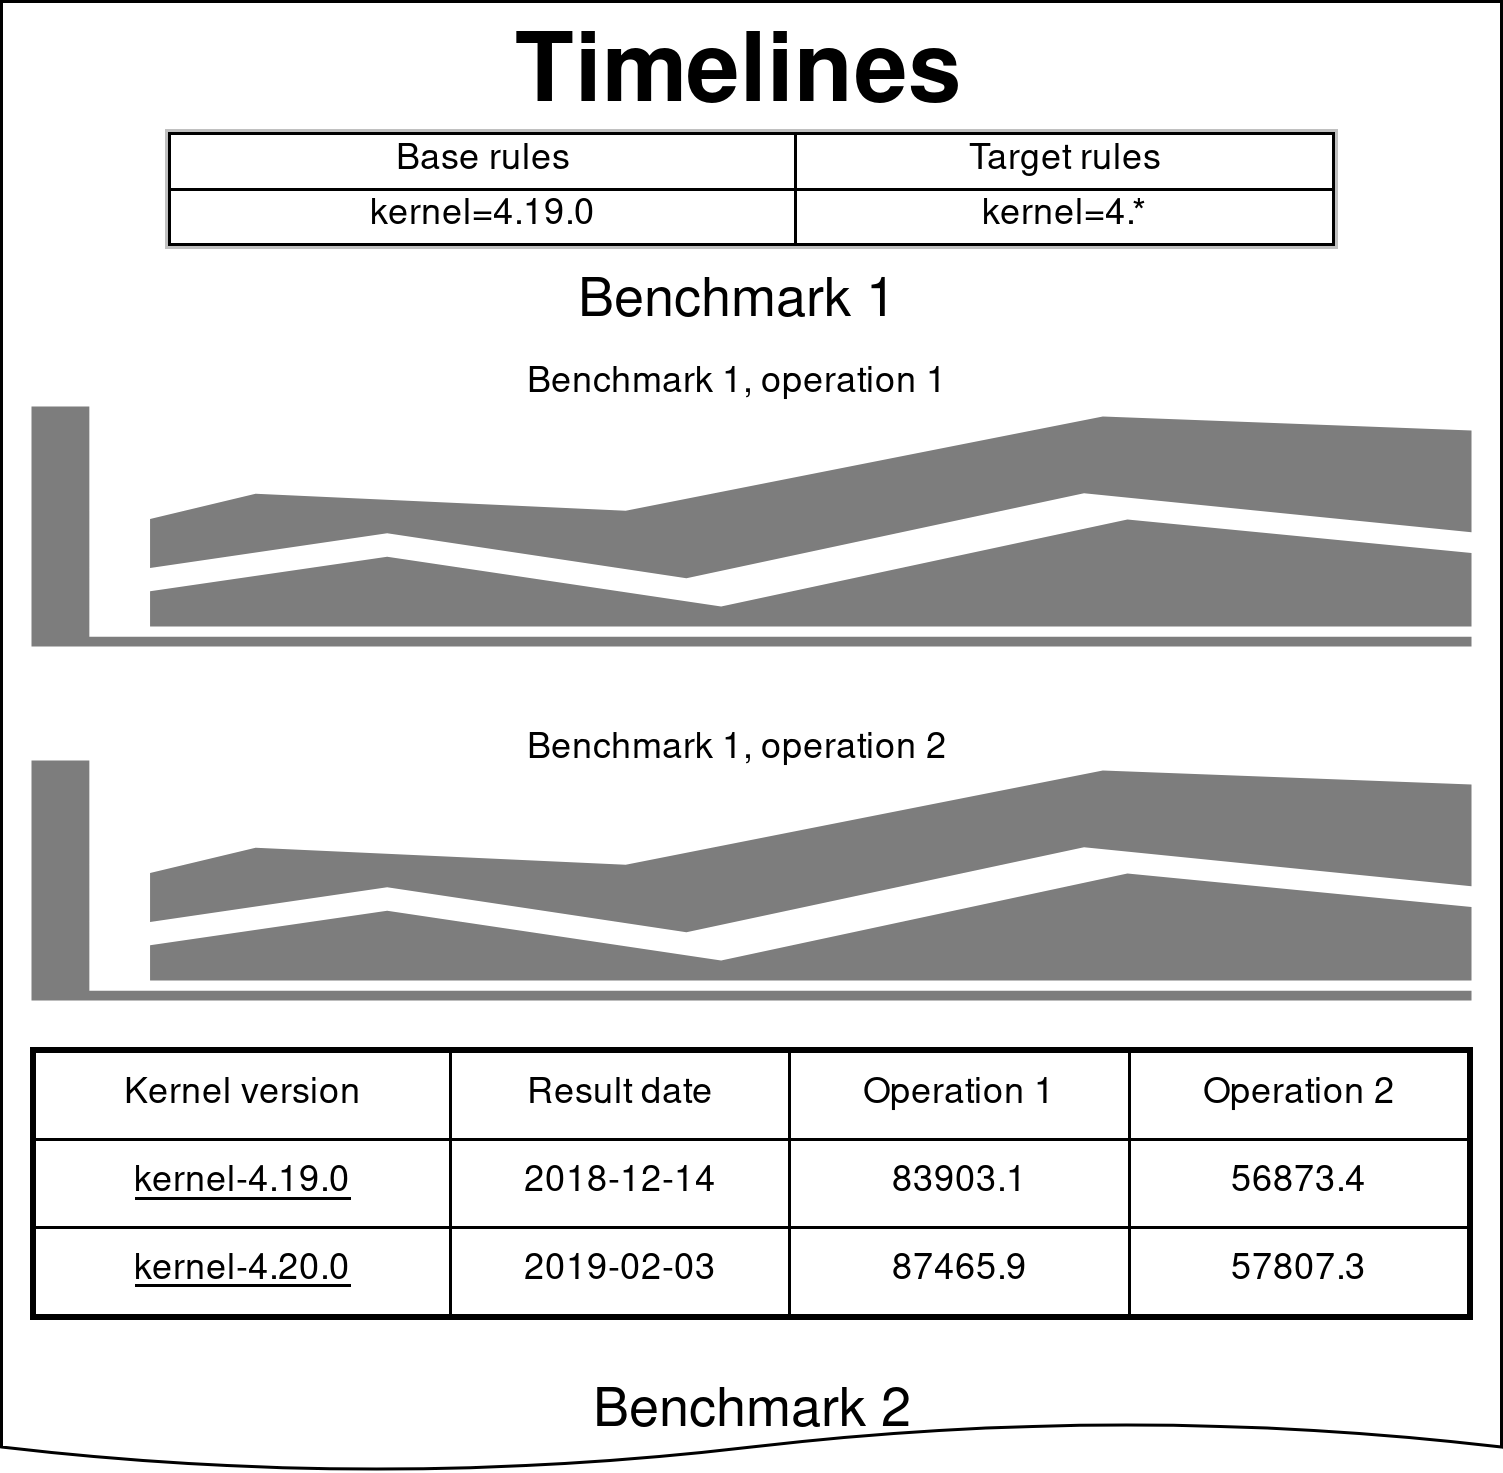
\includegraphics[width=8cm]{mockup}
  \caption{Mockup of timelines report page. The report will contain results from
    single testing machine fulfilling specified rules. Below table with the rules
    in the top of the report will be graphs of the available benchmarks. Each
    benchmark section will have separate graph for each of its operation and table
    below the graphs containing featured values from each operation for each
    benchmark with links to the results in our result database.}
  \label{fig:mockup}
\end{figure}

Best type of graph for results with repeated runs are boxplots. Boxplots show
important statistical values from the runs: median, minimum, maximum and first
and third quartiles. Those values will quickly reveal stability of plotted
benchmark and noise in the measurement helping with distinguishing of true
performance degradations.

Each graph of benchmark operation will contain results from all thread
configuration, but only one desired configuration will be visible by default.
The desired number of threads is the point where performance regressions create
biggest difference, which is in most cases the highest number of threads.

The graphs will also contain horizontal lines in background following median of
base result and its value increased and decreased by 5\%. Those lines will allow
more effective recognition of significant performance changes without looking at
the absolute values of the measurements.

Under the graphs of all operations of benchmark will be table containing medians
of featured thread runs for each benchmark operation of every displayed kernel
for browsing of the absolute result values. Each record will also work as link
to result record in our team database of benchmark results.

\section{Implementation}
This section describes aspects of implementation of the timelines report generator.
The programming for the generator was chosen Python2 due to earlier origins of
its implementation.

\subsection{Comparison rules}
For automatic report generation are essential rules, which will specify results,
that can be used and in which role. We propose to use \emph{regular expressions} to match
properties of results. Regular expressions offer broad possibilities to describe
shape of kernel version or just value of any environment configuration. E.g. to filter
all builds of kernel 4.18 we can use simple pattern \texttt{kernel-4.18\textbackslash
..*}.

We store the rules in an XML file with the same node naming as in the XML file
with the result properties. The first level of XML document contains three nodes
representing the purpose of the rules.
\begin{itemize}
  \item \textbf{Baseline rules} specify the first result in the plotted set.
    Acts as the main result that the others are compared to. In case of multiple
    results fitting the rule, the newest one will be used.
  \item \textbf{Target rules} define the results to be plotted.
  \item \textbf{Starting rules} are for the case, when base result is not from
    target set of results and specifying first target result with regex would be
    hard.
  \end{itemize}

\subsection{Reading of results}
Benchmark results are in our case stored on filesystem in directories. The
generator has to go recursively through directory with results of benchmark runs
with files containing desired data. From each result, it starts with file
containing properties of given result. This file provides metadata from the
benchmark run including the time, machine hostname, kernel and OS version,
benchmark name, configuration of environment for selecting desired results using
the comparison rules. Example of XML file with properties is in Figure
\ref{fig:xml_config}.

After applying the rules the generator reads files from
selected results with preprocessed data that are ready to use for drawing box
plot graphs. Example of the file with preprocessed values is in Figure
\ref{fig:xml_sums}. Parsed data from this XML file is all the generator needs to
start drawing the timeline graphs.

\subsection{Plotting of timelines}
For displaying the data in graphs using box plots we will use Highcharts
javascript library\;\cite{highcharts} for generating interactive SVG-based
graphs for HTML pages. It is offers free license for non-commercial use with
available source code, but also paid licenses for commercial use. It provides
fast and easy creation of various types of graphs including box plots with wide
possibilities of customization.

how are charts generated

\subsection{Generator parallelization}
usage of multiple processes
there is no need for locks - the common data are only read by the processes

\section{Generated output}
Example of timelines graphs

\begin{figure}
  \centering
  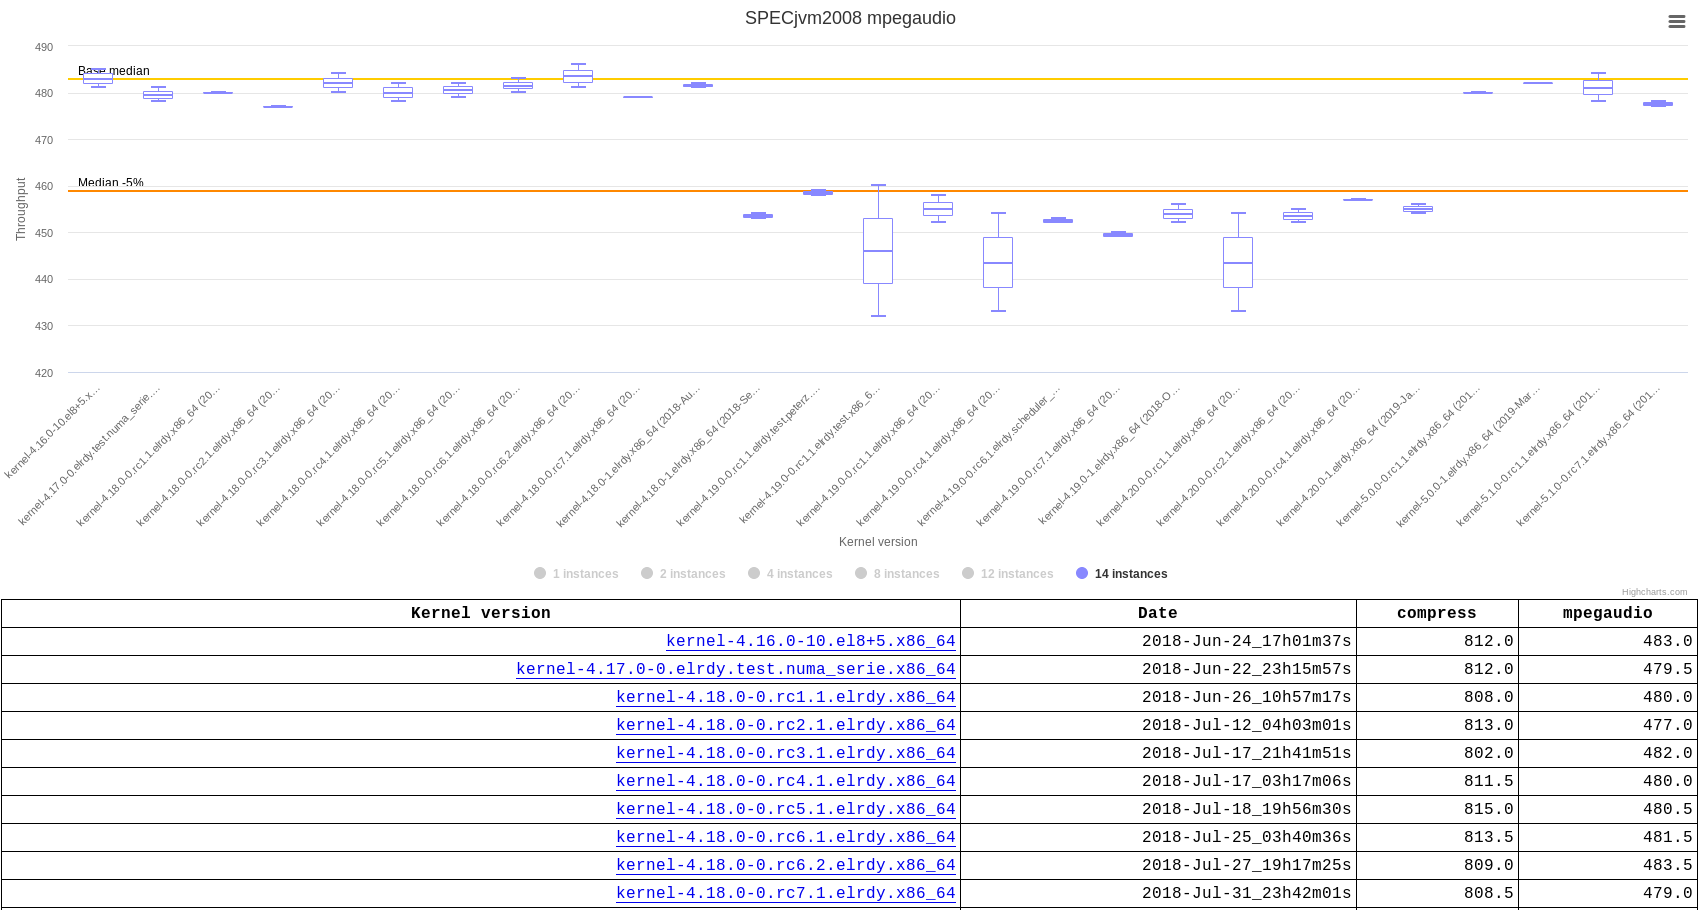
\includegraphics[width=15cm]{timeline_jvm_table}
  \caption{Generated box plot timeline graph of \emph{mpegaudio} operation from
    SPECjvm2008 benchmark with part of table showing numeric results of the
    SPECjvm2008 operations. The table shows medians from benchmark runs with
    featured number of threads and the kernel names are links to our team
    database of results. It displays performance results of upstream kernels for
    Red Hat Enterprise Linux 8. The performance degradation is consequence of
    changes in memory placement and migration behavior.}
  \label{fig:timeline_jvm_table}
\end{figure}

\begin{figure}
  \centering
  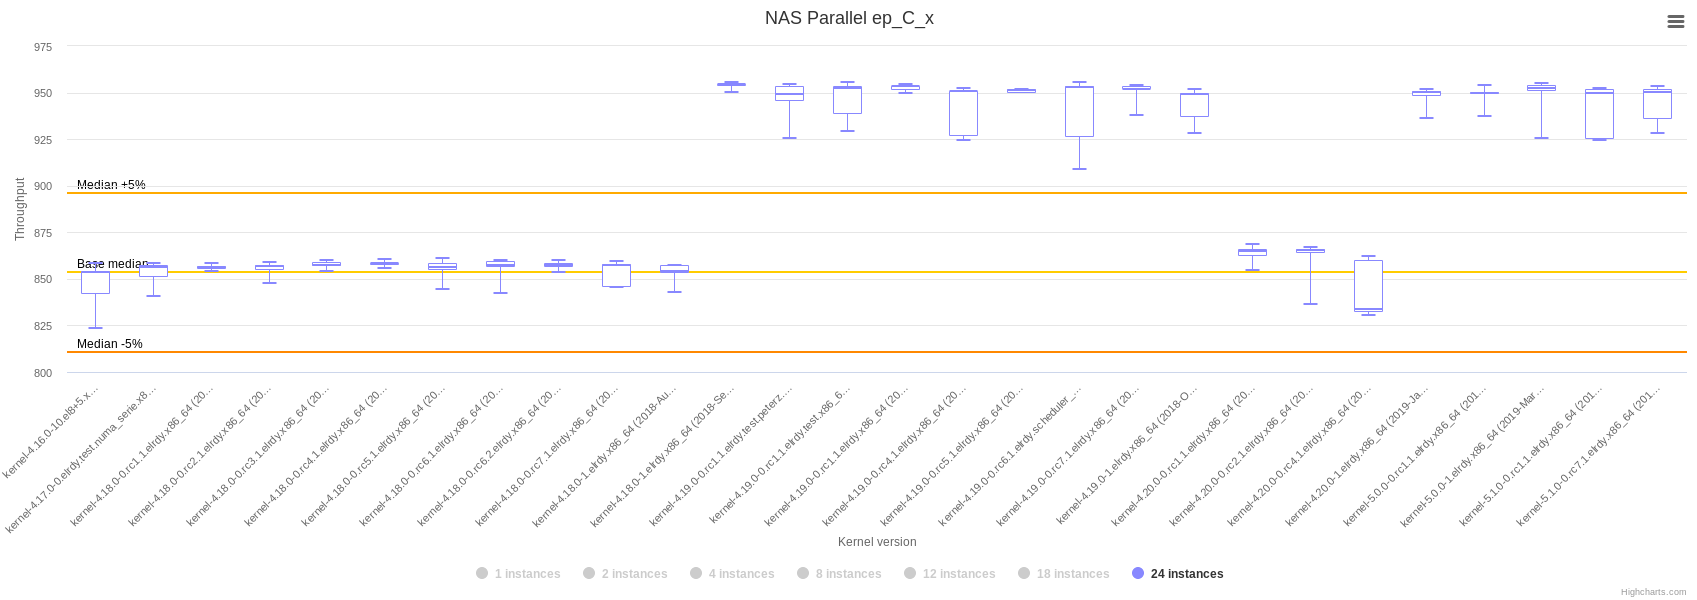
\includegraphics[width=15cm]{timeline_nas}
  \caption{Timeline box plot from the same report as Figure
    \ref{fig:timeline_jvm_table} showing results of \emph{Embarrassingly
    Parallel} operation from NAS Parallel benchmark. This benchmark got
    performance gain in the same version as the SPECjvm2008 benchmark registered
    performance degradation. Fortunately, this performance gain in NAS Parallel
    benchmark operation did not disappeared after fixing the degradation at
    SPECjvm2008 benchmark.}
  \label{fig:timeline_nas}
\end{figure}



\chapter{Automatic evaluation} \label{ch:ai}
With every new release of regular kernel and its testing the amount of produced
results rises. With more machines with different configurations, benchmarks with
different focus or baselines from different supported versions, number of results
can rise with every new kernel version even by hundreds.

In this thesis we attempt to automate the repetitive classification and
labeling of results as passed (without any performance regression) or failed
(containing performance regression). This allows skipping the results without
any significant change. Instead, more time is left for focusing on the results
with performance regressions.

In this chapter we will describe the way of obtaining data from results and
their processing for the evaluation. We will describe different classification
models suitable for given dataset and compare their success rate.

\section{Human classification of results}
There are quite many results to check with every new tested kernel. The test
suite with the Linpack, Stream, NAS Parellel and SPEC benchmarks are run on more
than eight machines with different amount of NUMA nodes and processor models.
Man has to go through the reports and check the results of all the benchmarks
with different configurations.

When looking at results of benchmark operation, the most important values are
medians from runs with different amount of threads. Unfortunately, due to noise in measurement
and limited amount of repeated runs the medians can be significantly affected by
the noise. This complication brings the need of more detailed inspection of
results than just watching difference in medians of results.

Another useful data are minimum, maximum and quartile values from each
measurement. They reveal the stability of the benchmark and the measurement
noise. With those values it is much easier and more accurate telling the
measurement noise from performance regression. With similar minimum, maximum and
quartile values the performance can be the same even with difference in median values.

The threshold between noise and performance regression is considered as 5\%
difference between base and target measurement but varies by the stability of
each benchmark and complexity of the machine it was run on.

\section{Used technologies}
For classification we use library \emph{scikit-learn}\;\cite{scikit-learn} with
Python3. Scikit-learn is a simple library for data analysis and machine learning
with BSD open source license. It is easy to use with fast learning curve and
well documented. It is a good choice for small and medium sized projects that do
not need massive scalability. It provides various algorithms for classification,
regression and clustering built on \emph{NumPy} and \emph{SciPy} Python
libraries.

Unlike other machine learning libraries like PyTorch and TensorFlow, the
scikit-learn library does not focus on deep neural networks for larger and
advanced problems. It provides more simple classifiers for easier problems
with smaller datasets where advanced methods would not have enough training
data.

\section{Reading the labeled results} \label{sec:learn_xml}
Learning data come as an XML file containing preprocessed data from
the base and the target run of the benchmark which are labeled as passed or failed.

Record of each benchmark operation is labeled as pass or fail and contains
records of runs with different amount of threads or processes. Those records
contain median, minimum, maximum and quartiles form the repeated runs of the
configuration. The root element contains UUIDs of the comparison and its base
and target results for easier tracing in case of suspicious values.

Example of XML file with data for the teaching of classifiers is shown in Figure
\ref{fig:learn_xml}.

\begin{figure}
  \small
  \begin{verbatim}
<comparison_results base_uuid="..." report_uuid="..." target_uuid="...">
  <comparison_result benchmark_name="NASParallel"
      operation_name="bt_C_x" result_status="pass">
    <result median_diff="1" threads_no="4">
      <base_result first_q="7409.2" max="7507.0" mean="7451.7"
        median="7456.5" min="7406.4" stdev="39.2" third_q="7479.3" />
      <target_result first_q="7503.0" max="7597.5" mean="7513.1"
        median="7522.2" min="7404.8" stdev="62.7" third_q="7537.8" />
    </result>
    <result median_diff="0" threads_no="8">
      <base_result first_q="14330.8" max="14740.1" mean="14476.6"
        median="14469.1" min="14325.9" stdev="151.7" third_q="14517.2" />
      <target_result first_q="14494.5" max="14619.3" mean="14481.1"
        median="14521.6" min="14233.7" stdev="130.5" third_q="14536.5" />
    </result>
...
  \end{verbatim}
  \normalsize
  \caption{Part of XML file with labeled data for classification.}
  \label{fig:learn_xml}
\end{figure}

\section{Labeling of results}
To teach the automatic classifier we need large amount of data for training. To
reduce the time spent on labeling of the passed and failed results we included a
HTML form to report page with comparison of two results to speed up this
process. The design of the form is shown in Figure \ref{fig:label_form}.

\begin{figure}
  \centering
  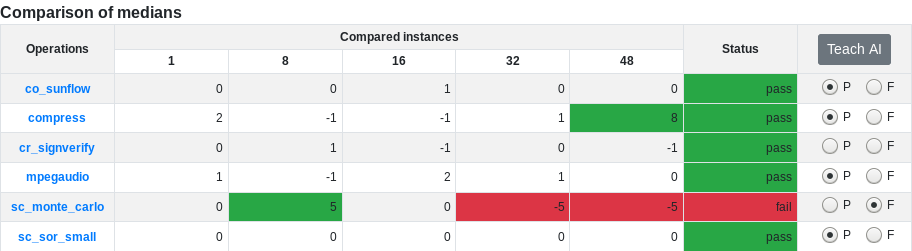
\includegraphics[width=12cm]{teaching_table}
  \caption{Form from HTML comparison report page to label data for machine learning}
  \label{fig:label_form}
\end{figure}

For processing of requests from the HTML form we built a simple HTTP simple
server application using Flask framework for Python3. It is wrapped in Docker
container which runs on machine which stores the performance results and
comparison reports. It receives a HTTP request with POST data containing type of
benchmark, path to directory with the report page and labels for results of each
benchmark operation. Using this data the application modifies the XML file with
labels described in Section \ref{sec:learn_xml} and returns HTTP redirect header
back to the comparison report. This process is shown in diagram in Figure
\ref{fig:marker_diagram}.

\begin{figure}
  \centering
  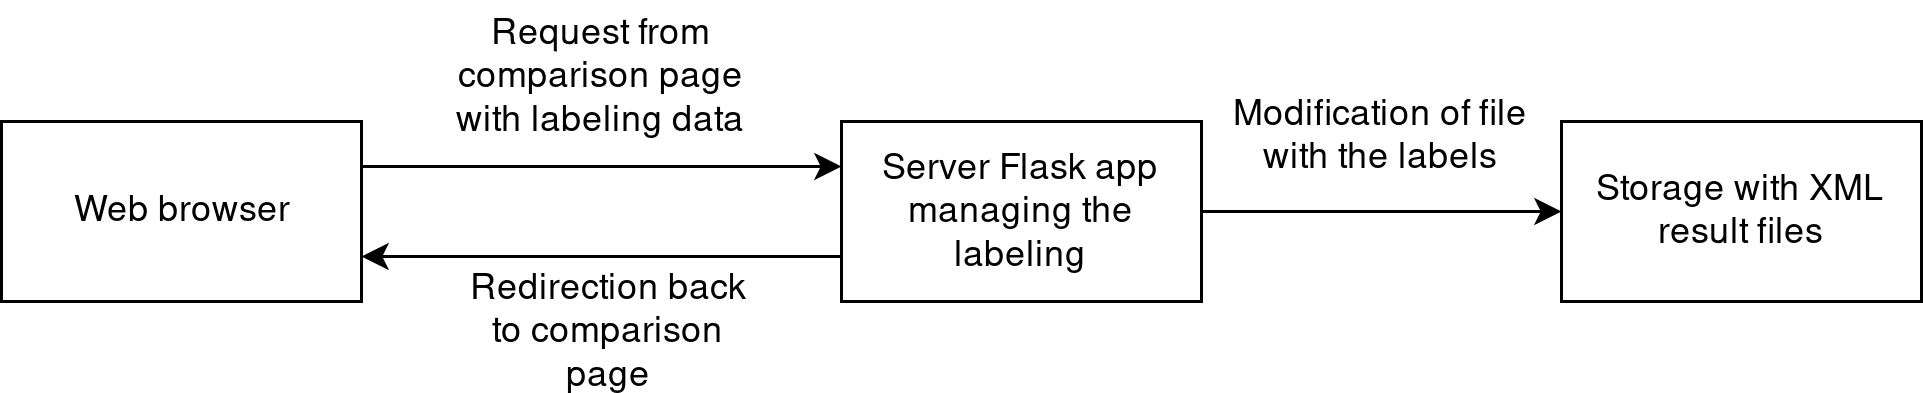
\includegraphics[width=12cm]{marker_diagram}
  \caption{Form from HTML comparison report page to label data for machine learning}
  \label{fig:marker_diagram}
\end{figure}

\section{Preprocessing for learning} \label{sec:learn_preprocess}
The intended task is to classify result of each benchmark operation with
different thread configurations which is represented by
\texttt{<comparison\_result>} node in example from previous section. The number
of threads configurations represented by \texttt{threads\_no} attribute in each
\texttt{<result>} is not always the same and varies on the number of CPU cores
on the testing machine.

The important values we focus on are the statistical data from runs with
different amount of threads, that a man uses to label the data manually. From
each of the runs we take minimum, median, maximum and first and third quartile
from the repeated measurements of the same run configuration.

To avoid absolute values from measurements that are different on each machine,
we will use relative proportions. Difference of target and base medians will be
divided by base median and the rest of target statistical values will be divided
by the target median.

Next task is to reduce provided data with variable number of threaded results
to fixed size vector. We will take minimum, median and maximum from values of
each statistical property: of minimums, medians, maximums and first and third
quartiles. This reduction will keep important values form the benchmark
operation results in reasonably small vector.

Last operation with vector values is applying square root on them. This
operation reduces distances of vectors with exceptionally high values, which
helps the k-NN and linear classifier to get better results. Scatter of the
vectors plotted in 3 best dimensions is shown in Figure \ref{fig:vectors_plot}.

For later use, we will name the vector component like \texttt{medians min} is
minimum value of all medians in results with different number of threads.

The whole preprocessing of a single result of benchmark operation shows the
Figure \ref{fig:learn_preprocess} with Python code snippet.

\begin{figure}
  \centering
  \includegraphics[width=14cm]{vectors_plot}
  \caption{In this figure are plotted vectors from the training dataset reduced
    to 3 dimensions, which are the best for classification. The reduction was done by
    \texttt{SelectKBest} class from scikit-learn library by choosing the
    dimensions with the biggest variability between classes. The plot on the
    left shows scatter of vectors from dataset with unmodified values. The plot
    on the right shows the vectors from dataset modified by applying square root
    on their values. This modification and naming of the axis is explained in
    Section \ref{sec:learn_preprocess}}
  \label{fig:vectors_plot}
\end{figure}

\begin{figure}
  \small
  \begin{lstlisting}[language=Python]
mins = []
medians = []
maxes = []
q1s = []
q3s = []

# Iterate over the thread results of single benchmark operation
for res in cpresult:
    for basetarget in res:
        if basetarget.tag == "base_result":
            b_attr = basetarget.attrib
        if basetarget.tag == "target_result":
            t_attr = basetarget.attrib
    try:
        medians.append((float(t_attr["median"]) - float(b_attr["median"]))
                        / float(b_attr["median"]))
        mins.append((float(t_attr["median"]) - float(t_attr["min"]))
                        / float(t_attr["median"]))
        maxes.append((float(t_attr["median"]) - float(t_attr["max"]))
                        / float(t_attr["median"]))
        q1s.append((float(t_attr["median"]) - float(t_attr["first_q"]))
                        / float(t_attr["median"]))
        q3s.append((float(t_attr["median"]) - float(t_attr["third_q"]))
                        / float(t_attr["median"]))
    except:
        print("ERROR in values in " + path)

vector = []
for a in [medians, mins, maxes, q1s, q3s]:
    vector.append(min(a))
    vector.append(median(a))
    vector.append(max(a))

vector = list(map(lambda x: math.sqrt(float(x))
                  if float(x) > 0
                  else -math.sqrt(abs(float(x))), vector)))
  \end{lstlisting}
  \normalsize
  \caption{}
  \label{fig:learn_preprocess}
\end{figure}
% TODO describe the code

\section{Comparison of classifiers} \label{sec:classifier_comparison}
Classification is procedure of assigning category to new observation based on
training set of observations with specified category. Because of the
availability of already classified data it belongs to \emph{supervised learning}
part of machine learning.

Data for classification are represented by set of vectors with fixed element
count. Vector is an ordered set of numbers where each one represents a value in
separate dimension of the source data. For supervised learning have vectors from
training set assigned categories (also called classes). In our case we will have
2 classes: \emph{pass} and \emph{fail}.

For the following training and evaluation of the models we have roughly 250
labeled vectors. This should be enough to train different simple classifiers with
sufficient accuracy on other unlabeled vectors.

\subsection{Validation and metrics}
To compare success rate of different classification models we need a method to evaluate
accuracy of predicting new data. Testing the model on data it got also for
learning brings risk of overlooking \emph{overfitting}. Overfitting means that the model
precisely predicts data it has already seen, but fails to predict any new data
it has not seen yet.

To avoid overfitting we will use \emph{cross-validation} method to test model.
It removes part of data from training set and uses them as testing set for
evaluating the prediction.

For splitting the training data we will use \emph{k-fold} method. This method
splits the original dataset to $k$ groups. One of groups is used as testing set and
the rest $k - 1$ groups are left for training. This way we get $k$ different
dataset for evaluation of our classifiers.

As implementation of k-fold cross-validation we will use
\texttt{RepeatedStratifiedKFold} class from scikit-learn library with parameter
$k$ set to 4. It will split the original dataset to 4 groups with same ratio of
pass and fail labels repeating this process with differently shuffled data.
Setting number of folds to 4 will give us enough data for training, but also for
the evaluation.

As metric for rating of predicted values we will use \emph{accuracy} scoring.
Predicted results will be evaluated as 1 or 0 if the predicted class is the same as the reference
class from manual labeling or not. Averaging those scores from the whole testing
set will give us ratio of correctly predicted vectors.

\subsection{k-nearest neighbors classifier}
This classifier does not construct any generalized model, but works with the
whole training data. The decision is made by voting of the $k$ nearest
neighbors.

The learning process consists only of building data structure for more efficient
search through the learning dataset. More computations come with the prediction
when the algorithm must go through the learning dataset and find $k$ nearest
vectors.

Accuracy of the model highly depends on the parameter $k$. Higher values
suppress noise in dataset, but can smoother the boundaries of classes too much.
This behavior can be seen in Figure \ref{fig:knn}.

Scikit-learn implements k-NN classifier in \texttt{KNeighborsClassifier} class.
Next to setting the $k$ number it provides parameter for weighting votes. First
option is uniform voting where each of the $k$ neighbors have the same weight of
the vote. The second option weights votes based on the distance from queried
vector. The weighted option provides better results for our dataset as can be
seen in Figure \ref{fig:knn}.

\begin{figure}
  \centering
  \includegraphics[width=14cm]{knn}
  \caption{Accuracy of k-nearest neighbors classifier on available training
    data with different parameters. On x axis is number of k-nearest neighbors
    that vote for the class of queried vector. The two plotted lines differ in
    weighting of the votes. The first takes all votes with uniform weight and
    the second weights the votes by distance of the neighbors from the queried
    vector.}
  \label{fig:knn}
\end{figure}

\subsection{Linear classifier}
Linear models try to separate vectors of two different classes to two spaces
using a line, plane, hyperplane, etc. depending on the dimensionality of the
vectors.
\ref{fig:vectors_plot}

\subsection{Decision tree classifier}
Decision of this classifier is based on decision tree built on training data.
In each node the tree looks on one component of the queried vector and by
comparison with learned threshold the tree decides to which branch it will
continue. Each leaf of the tree contains label that is returned for the queried
vector which led to the leaf.

Learning of the model involves the construction of the decision tree. The
construction looks for the best component of vector for splitting the dataset by
classes. It creates a decision node and splits the training dataset based on the
selected component to the decision branches. This process is recursively
repeated with each part of the split dataset until the split contains vectors of
single class (purity of the node is 1) or any additional restrictive condition
is met.

Main advantage of the decision tree is its transparency and easy visualization
of the model. In Figure \ref{fig:decision_tree} there is visualization of
decision tree constrained by depth and samples count in leaf nodes built with
our dataset of performance comparisons.

Disadvantage of the decision tree is sensitivity to noisy data and is high
chance of overfitting, because the tree tries to fit the whole dataset and has
100\% prediction accuracy on already seen data. This issue can be suppressed by
reducing maximum depth of the tree, setting minimal amount of samples required
to split impure node into another decision.

\begin{figure}
  \centering
  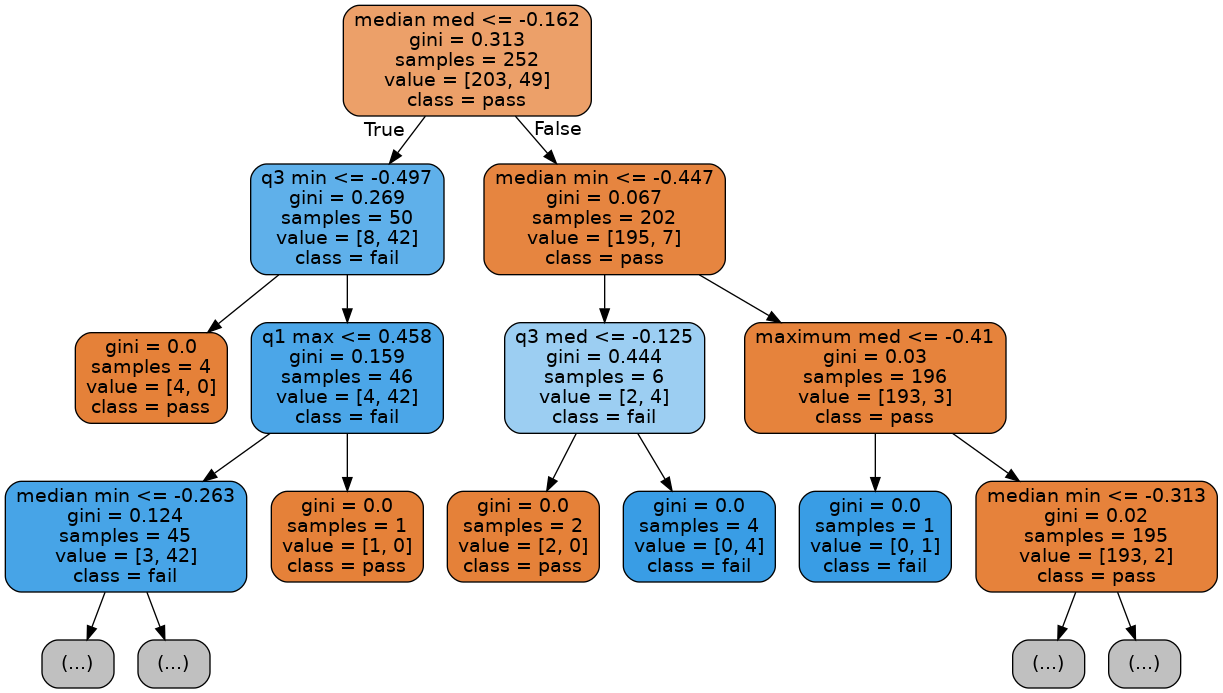
\includegraphics[width=14cm]{decision_tree}
  \caption{Decision tree created by Decision tree classifier and rendered by
    Graphviz library for Python. It shows decision tree generated on our
    performance comparison data constrained by depth and samples count in leaf
    node. First line of non-leaf node shows the condition for choosing the next
    decision branch. \emph{gini} property of node shows its impurity --
    proportion of training data not fitting the class of the node. Leaf nodes
    have 0 impurity because they contain vectors of single class. Parameters
    \emph{samples} and \emph{value} show the amount of training vectors for the
    subtree and their division to pass and fail classes.}
  \label{fig:decision_tree}
\end{figure}

\subsection{Forest of randomized trees classifiers}
The forest of randomized trees classifier extends the decision tree
classification by creating a set of decision tree classifiers with small portion
of randomness introduced in the creation of the decision trees. Output of the
classifier is decided by voting of the decision tree classifiers. This
modification compensates the overfitting of single decision tree classifiers.
Although the amount of trees slightly increases the accuracy of the prediction,
the duration of learning of the model and prediction rises linearly with the
amount of trees.

The scikit-learn library provides two implementation of classifiers based on
randomized trees. The first is \texttt{RandomForestClassifier} class. The
dataset for each tree is resampled with replacement creating slightly reduced
and different dataset. When building a decision tree, the component used for
comparison in the node is not the best for splitting, but randomly chosen.

The second is extremely randomized trees method implemented in
\texttt{ExtraTreesClassifier} class. This implementation extends the randomness
by choosing more thresholds for decision randomly and selecting the best instead
of computing the most discriminative one. This method helps to reduce variance
of the model at the cost of higher bias.

Comparison of these two implementations is in Figure
\ref{fig:randomized_forests}. The RandomForestClassifier has slightly better
accuracy than ExtraTreesClassifier. Accuracy also rises much slower compared to
number of the trees in the model.

\begin{figure}
  \centering
  \includegraphics[width=14cm]{randomized_forests}
  \caption{Accuracy of randomized forests classifiers on available training
    dataset with different parameters. On x axis is number of trees that vote
    for the class of queried vector. The first plotted line represents the
    Random forest method and the second the Extra trees method of building the
    trees.}
  \label{fig:randomized_forests}
\end{figure}

\section{Evaluation of classifiers}
What is cross validation
Best classifiers seems to be knn and random forest.
This classifier will be added to analyzer for automatic labeling of comparisons.

\begin{figure}
  \centering
  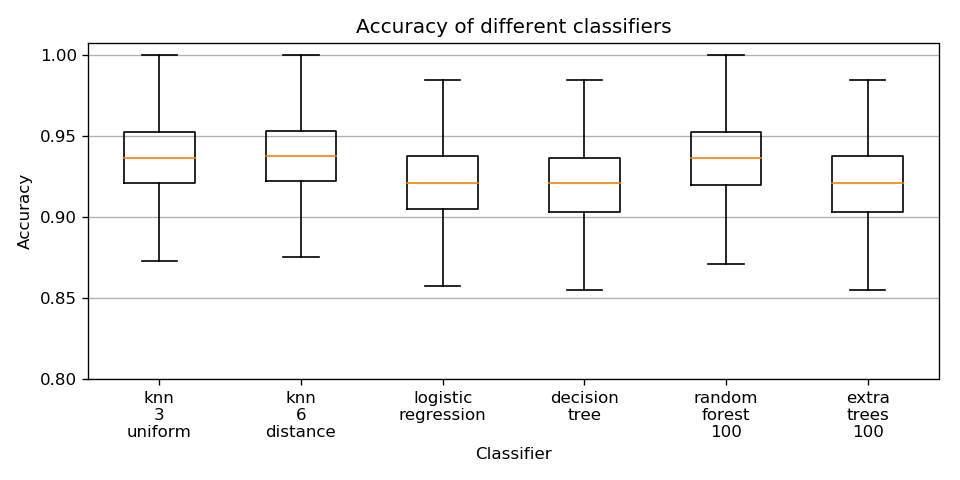
\includegraphics[width=14cm]{classifiers}
  \caption{Comparison of accuracy of different classifiers mentioned in Section
    \ref{sec:classifier_comparison}. The results come from cross-validation by
    split the dataset to train and test sets using ratio 3:1.}
  \label{fig:classifiers}
\end{figure}



\chapter{Future work}
more precise classification with more learning data
classification of results can be included to timelines



\chapter{Conclusion}
In this work we described ...
... was evaluated ...

Závěrečná kapitola obsahuje zhodnocení dosažených výsledků se zvlášť vyznačeným
vlastním přínosem studenta. Povinně se zde objeví i zhodnocení z pohledu dalšího
vývoje projektu, student uvede náměty vycházející ze zkušeností s řešeným
projektem a uvede rovněž návaznosti na právě dokončené projekty (řešené v rámci
ostatních bakalářských prací v daném roce nebo na projekty řešené na externích
pracovištích).


\chapter{Notes}
\begin{verbatim}
zkontrolovat prekladatelem
zminit Red Hat
citovat cely scikit, nebo konkretni stranky
vlozit nedelitelne mezery
stress more what is my work, team and general knowledge
  in our team we use ..., my part of work is ...
klicova slova v lstlisting
jednostranny tisk
rozsirit podekovani

text semestralni prace
licence zdrojaku
lstlisting na jednu stranu
timeliny jako section vizualizace?
(1) a (2) v introductionu

Linux scheduler
    manual pinning option
        numactl
    group imbalance bug
    tuned profiles
        focus on throughput or latency
Performance
    provisioning of machines with Beaker
    collecting system load data
        numastat
        numatop
            usage of cpu and memory on each node
        perf stat
        lstopo for hardware schema image
        free
    scenarios
        variable number of benchmark instances
        with and without pinning processes to specific numa nodes
    result storing
        preprocessing to xml
        storing to database
        aggregating results
        computing statistical data
    plotting
        lstopo for plotting hardware topology
        bargraphs to show inaccuracy
            operations per second (run time of benchmark)
            time out of cpu
        detailed comparison of two results
        timeline with many results over longer period of time
\end{verbatim}